%============================================================
\section{Nombre: Tornado.} \label{hab.tornado}
\subsection{Descripción}
Poderoso ataque que puede bajar hasta la mitad de la vida del jugador. El enemigo se rodea de un poderoso tornado. El tonado atraerá al jugador hacia él. El tornado disminuirá la cantidad de vida del jugador de manera constante mientras el jugador se mantenga en colisión con el tornado. El tornado desaparecerá después de un tiempo y mientras se mantenga activo el enemigo no podrá recibir daño por el disparo de tonalli del jugador.
\subsection{Portador}
Mictlecayotl (ver apartado \ref{per:mictlecayotl}).
\subsection{Esquema}
			Ver figura \ref{fig:tornado}.
			\begin{figure}
				\centering
				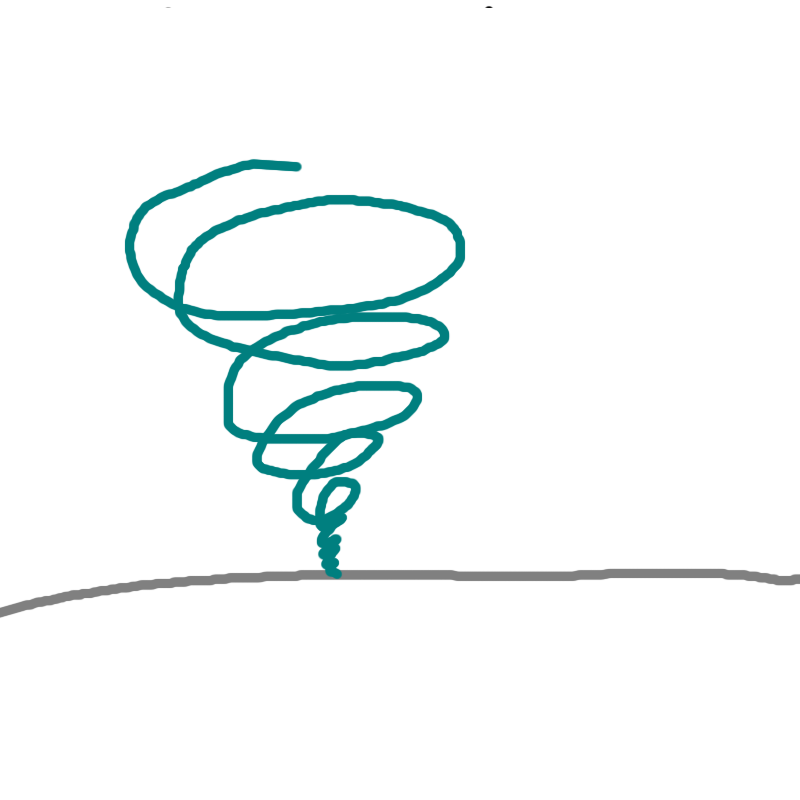
\includegraphics[height=0.2 \textheight]{Imagenes/tornado}
				\caption{Tornado.}
				\label{fig:tornado}
			\end{figure}